\documentclass[3p,times]{elsarticle}

\usepackage[utf8]{inputenc}
\usepackage[T1]{fontenc}
\usepackage{amsmath,amssymb,amsthm}
\usepackage{algorithm}
\usepackage{algpseudocode}
% algpseudocode does not define switch/case out of the box.
\algnewcommand{\Switch}[1]{\State \textbf{switch} #1}
\algnewcommand{\Case}[1]{\State \textbf{case} #1}
\algnewcommand{\EndCase}{}
\algnewcommand{\EndSwitch}{}
\usepackage{tikz}
\usetikzlibrary{calc,patterns,decorations.pathmorphing,arrows.meta,positioning}
\usepackage{xcolor}
\usepackage{hyperref}
\usepackage{cleveref}
\usepackage{multirow}
\usepackage{booktabs}
\usepackage{url}
\usepackage{placeins}

% Avoid duplicate hyperlink anchors for algorithmic line numbers when multiple
% algorithms appear in the paper (hyperref otherwise reuses ALG@line.1, etc.).
\makeatletter
\providecommand{\theHalgorithm}{\arabic{algorithm}}
\providecommand{\theHALG@line}{}
\renewcommand{\theHALG@line}{ALG@line.\thealgorithm.\arabic{ALG@line}}
\makeatother

\newtheorem{theorem}{Theorem}
\newtheorem{lemma}[theorem]{Lemma}
\newtheorem{corollary}[theorem]{Corollary}
\newtheorem{proposition}[theorem]{Proposition}
\theoremstyle{definition}
\newtheorem{definition}[theorem]{Definition}
\newtheorem{remark}[theorem]{Remark}

\definecolor{polyblue}{RGB}{70,130,180}
\definecolor{diagred}{RGB}{180,60,60}
\definecolor{chaingreen}{RGB}{60,140,60}

\journal{Computational Geometry: Theory and Applications}

\begin{document}

\begin{frontmatter}

\title{A Simple, Practical, and Fast Polygon Triangulation in \texorpdfstring{$O(n + k\log k)$}{O(n + k log k)} Time}

\author[knu]{Pavel Shpagin\corref{cor1}}
\ead{pavelandrewshpagin@knu.ua}
\author[knu]{Vasyl Tereschenko}
\cortext[cor1]{Corresponding author}
\address[knu]{Faculty of Computer Science and Cybernetics, Taras Shevchenko National University of Kyiv, Kyiv, Ukraine}

\begin{abstract}
We present a practical algorithm for triangulating a simple polygon with $n$ vertices in $O(n + k\log k)$ time, where $k$ is the number of local extrema with respect to the sweep direction.
The key idea is a chain-based reformulation of the monotone-decomposition sweep: the sweep maintains active monotone chains rather than individual edges and advances chain pointers lazily, so all regular vertices cost $O(n)$ total while balanced-tree work is confined to $O(k\log k)$ over the $2k$ extrema.
We evaluate against state-of-the-art practical triangulation pipelines with publicly available implementations, including Garey et al., Seidel, and Hertel--Mehlhorn, and find that our method is faster across all tested families, with large speedups on nearly convex inputs.
\end{abstract}

\begin{keyword}
simple polygon \sep triangulation \sep monotone decomposition \sep input-sensitive algorithm \sep plane sweep
\end{keyword}

\end{frontmatter}

%==============================================================================
\section{Introduction}
\label{sec:intro}
%==============================================================================

Triangulating simple polygons is a fundamental problem in computational geometry. Chazelle~\cite{chazelle1991} proved that $O(n)$ time is achievable, but the algorithm's complexity has limited practical adoption. The plane sweep of Garey et al.~\cite{garey1978}, running in $O(n\log n)$ time via monotone decomposition, remains standard; see de Berg et al.~\cite{deberg2008}. Seidel~\cite{seidel1991} gave a simplified randomized $O(n\log^* n)$ expected-time algorithm.

We present an algorithm running in $O(n + k\log k)$ time, where $k$ is the number of local extrema with respect to the sweep direction. This interpolates between $O(n)$ for convex polygons ($k = 1$) and $O(n\log n)$ for worst-case polygons ($k = \Theta(n)$), and can improve upon classical methods when $k$ is substantially smaller than $n$.
We show in \Cref{sec:complexity} that \(k \le r + 1\), where \(r\) is the number of reflex vertices, so the bound also implies \(O(n + r\log r)\).

The key observation is that the sweep needs to process only local extrema, and regular vertices can be handled implicitly by advancing chain pointers lazily. This yields $O(k)$ sweep events and $O(n)$ total pointer advancement, with balanced-tree operations totaling $O(k\log k)$.

Beyond the improved bound, the method is deliberately simple: it follows the classical monotone-decomposition sweep with the same event order and tie-breaking, but represents the status structure by monotone chains and advances along chains lazily. In \Cref{sec:experiments}, our implementation is faster than the standard Garey et al.\ pipeline across all tested polygon families and sizes, suggesting a new practical baseline for polygon triangulation. For clarity, we assume general position in the analysis; the implementation resolves equal $y$-coordinates by a deterministic lexicographic tie-break.

\paragraph{Related work}
The ear-clipping method is among the oldest practical triangulation algorithms; for smaller inputs, its $O(n^2)$ complexity~\cite{elgindy1985} is still attractive due to its simplicity. The classical plane sweep of Garey et al.~\cite{garey1978} decomposes a polygon into $y$-monotone pieces and triangulates each in linear time, achieving $O(n\log n)$ overall; see de~Berg et al.~\cite{deberg2008}. Triangulation of monotone polygons, the linear-time subroutine underlying this pipeline, goes back at least to Fournier and Montuno~\cite{fournier1984}.

Several works relate running time to geometric properties of the input. Hertel and Mehlhorn~\cite{hertel1983} gave a sweep whose cost depends on the number of start vertices $s$ and runs in $O(n + s\log s)$; for simple polygons, $s \le r+1$. Chazelle and Incerpi~\cite{chazelle1984} study triangulation under shape-complexity measures. Toussaint~\cite{toussaint1990,toussaint1991} gives output-sensitive triangulation algorithms. Our parameter $k$ counts local extrema in the sweep direction; \Cref{sec:complexity} shows \(k \le r+1\) and it can be strictly smaller than \(r\) when many reflex vertices are regular.

Worst-case bounds in $n$ have also been improved. Tarjan and Van~Wyk~\cite{tarjan1988} achieved $O(n\log\log n)$ using sophisticated data structures, later simplified by Kirkpatrick et al.~\cite{kirkpatrick1992}. Randomized incremental approaches proved fruitful: Clarkson et al.~\cite{clarkson1989} gave an $O(n\log^* n)$ expected-time Las Vegas algorithm, which Seidel~\cite{seidel1991} simplified significantly via trapezoidal decomposition. The breakthrough came with Chazelle's~\cite{chazelle1991} deterministic $O(n)$ algorithm, but its complexity has limited practical adoption; Amato et al.~\cite{amato2001} provided further simplifications to the randomized approach. Keil~\cite{keil2000} surveys polygon decomposition more broadly.

Since both monotone decomposition and the extrema count $k$ depend on the sweep direction, the choice of direction matters; Shin and Kim~\cite{shin2004} study selecting directions that optimize monotone-chain decompositions.

Our contribution is a deterministic chain-based reformulation of monotone decomposition that makes an extrema parameter \(k\) explicit in both the analysis and the implementation: the sweep performs balanced-tree work only at the \(2k\) extremal events, while all regular vertices are handled via amortized pointer advancement along chains.
For correctness, we prove equivalence to the classical helper-based monotone-decomposition sweep (see, e.g., de Berg et al.~\cite{deberg2008}): under the same event order and tie-breaking, our chain-based sweep produces the same decomposition diagonals.

\paragraph{Organization}
\Cref{sec:prelim} defines vertex types, monotone chains, left-boundary chains, and the event-complexity parameter $k$. \Cref{sec:algorithm} presents the algorithm. \Cref{sec:correctness} establishes correctness. \Cref{sec:complexity} analyzes complexity and relates $k$ to the reflex count $r$. \Cref{sec:experiments} provides experimental evaluation. \Cref{sec:discussion} discusses extensions.

%==============================================================================
\section{Preliminaries}
\label{sec:prelim}
%==============================================================================

Let $P$ be a simple polygon with vertices $v_0, v_1, \ldots, v_{n-1}$ listed in counterclockwise order along the boundary $\partial P$. We write $v_i = (x_i, y_i)$ for the coordinates of each vertex and adopt the convention that indices are taken modulo $n$, so $v_{-1} = v_{n-1}$ and $v_n = v_0$. The \emph{interior angle} at vertex $v_i$ is the angle $\angle v_{i-1} v_i v_{i+1}$ measured inside $P$. A vertex is \emph{convex} if its interior angle is at most $\pi$ and \emph{reflex} if its interior angle strictly exceeds $\pi$. We denote by $r$ the number of reflex vertices.

\begin{definition}[Vertex classification]
\label{def:vertex-types}
Assuming general position (no two vertices share the same $y$-coordinate), each vertex $v_i$ is classified according to the relative $y$-coordinates of its neighbors:
\begin{itemize}
\item \textbf{Start vertex:} $y_{i-1} < y_i$ and $y_{i+1} < y_i$, with interior angle $< \pi$.
\item \textbf{Split vertex:} $y_{i-1} < y_i$ and $y_{i+1} < y_i$, with interior angle $> \pi$.
\item \textbf{End vertex:} $y_{i-1} > y_i$ and $y_{i+1} > y_i$, with interior angle $< \pi$.
\item \textbf{Merge vertex:} $y_{i-1} > y_i$ and $y_{i+1} > y_i$, with interior angle $> \pi$.
\item \textbf{Regular vertex:} exactly one neighbor has $y$-coordinate greater than $y_i$.
\end{itemize}
\end{definition}

Start and split vertices are \emph{local maxima}; end and merge vertices are \emph{local minima}. Split and merge vertices are precisely the reflex vertices among local extrema. Regular vertices partition into two subtypes based on whether the polygon interior lies to their left or right as one traverses the boundary; this distinction is needed in \textsc{Advance} to mirror the classical sweep's regular-vertex behavior, but it does not affect the asymptotic bounds.

\begin{definition}[Monotone chain]
\label{def:chain}
A \emph{$y$-monotone chain} is a maximal contiguous sequence of boundary vertices whose $y$-coordinates are strictly monotonic (strictly increasing or strictly decreasing) along the chain. Each chain connects a local maximum to a local minimum.
\end{definition}

The boundary $\partial P$ decomposes uniquely into monotone chains, with consecutive chains sharing their endpoint extrema. Let $k$ denote the number of local extrema (maxima or, equivalently, minima) with respect to the sweep direction; then there are $2k$ chains, and $k$ controls the number of sweep events in our formulation.

\begin{definition}[Left-boundary chain]
\label{def:left-boundary}
A monotone chain is a \emph{left-boundary chain} if, when traversed from its upper endpoint to its lower endpoint, the polygon interior lies to the right of the traversal direction. Equivalently, for a counterclockwise-oriented polygon, a chain is left-boundary if its traversal direction (downward) opposes the boundary orientation.
\end{definition}

At each local maximum, exactly one of the two originating chains is left-boundary; at each local minimum, exactly one of the two terminating chains is left-boundary.

%==============================================================================
\section{Algorithm}
\label{sec:algorithm}
%==============================================================================

The algorithm consists of three phases: (1) chain construction and vertex classification, (2) monotone decomposition via chain-based plane sweep, and (3) triangulation of monotone pieces. We describe each phase in detail.

%------------------------------------------------------------------------------
\subsection{Phase 1: Chain Construction}
\label{sec:chain-construction}
%------------------------------------------------------------------------------

A single traversal of $\partial P$ classifies each vertex according to \Cref{def:vertex-types} and partitions the boundary into monotone chains. For each vertex $v_i$, we compare $y_i$ to $y_{i-1}$ and $y_{i+1}$ and compute the cross product $(v_{i+1} - v_i) \times (v_i - v_{i-1})$ to determine convexity. Simultaneously, we record each chain as an array of vertex indices from its upper endpoint (local maximum) to its lower endpoint (local minimum), and identify the incident left-boundary chain at each extremum (\Cref{def:left-boundary}). This phase runs in $O(n)$ time and produces $O(k)$ chains.

%------------------------------------------------------------------------------
\subsection{Phase 2: Monotone Decomposition}
\label{sec:decomposition}
%------------------------------------------------------------------------------

A polygon is \emph{$y$-monotone} if every horizontal line intersects it in a connected set (either empty, a point, or a segment). Split vertices violate monotonicity by creating local maxima where the boundary diverges downward; merge vertices violate it by creating local minima where boundary paths converge from above. The decomposition phase inserts diagonals to eliminate all split and merge vertices, partitioning $P$ into $y$-monotone subpolygons.

\paragraph{Sweep-line status structure}
Unlike the classical algorithm, which maintains individual edges in a balanced search tree $T$, we maintain \emph{active left-boundary chains}. A chain $C$ is \emph{active} at sweep height $y$ if $y$ lies strictly between the $y$-coordinates of $C$'s upper and lower endpoints. The tree $T$ stores active left-boundary chains ordered by their $x$-coordinate at the current sweep height.

Each chain $C$ in $T$ maintains:
\begin{enumerate}
\item \textbf{Edge pointer} $C.\mathit{curr}$: initialized to the topmost edge of $C$, this pointer tracks our position within the chain. The upper vertex of $C.\mathit{curr}$ serves as the \emph{slab entry}---the default diagonal target when no pending merge exists.
\item \textbf{Pending merge} $C.\mathit{pending}$: either null or a merge vertex awaiting connection to a lower vertex. When a merge vertex $v$ is processed and $C$ is immediately to $v$'s left, we set $C.\mathit{pending} \gets v$.
\end{enumerate}

\paragraph{Lazy edge pointer advancement}
The comparison function for $T$, when comparing chains at sweep height $y$, first advances each chain's edge pointer to ensure the current edge spans $y$:
\begin{algorithmic}[1]
\Procedure{Advance}{$C, y$}
    \While{$C.\mathit{curr}.\mathit{lower}.y > y$}
        \State $C.\mathit{curr} \gets$ next edge down $C$
        \State $u \gets C.\mathit{curr}.\mathit{upper}$ \Comment{vertex just passed}
        \If{$u$ is regular and $C.\mathit{pending} \neq \textsc{null}$ and $\mathsf{InteriorRight}(u)$}
            \State $D \gets D \cup \{(u, C.\mathit{pending})\}$; $C.\mathit{pending} \gets \textsc{null}$
        \EndIf
    \EndWhile
\EndProcedure
\end{algorithmic}
Here $\mathsf{InteriorRight}(u)$ is the standard regular-vertex side test from the classical sweep (i.e., the subtype of regular vertices handled like an end vertex); it can be decided from the local boundary configuration at $u$.
In \Cref{alg:decompose}, before inspecting a chain's fields at event vertex $v$ we call \textsc{Advance} on that chain at height $y(v)$; balanced-tree comparisons may also invoke \textsc{Advance} as needed.
After advancement, the $x$-coordinate of $C$ at height $y$ is computed by linear interpolation along $C.\mathit{curr}$. Since each vertex is visited by at most one chain's pointer exactly once, the total cost of all pointer advancements (and any diagonals emitted inside \textsc{Advance}) is $O(n)$, amortized over all tree operations.

\paragraph{Event processing}
The sweep processes local extrema in decreasing $y$-order. Let $E$ denote the sorted list of extrema; $|E| = 2k$, where $k$ is the number of local extrema.

\begin{algorithm}[H]
\caption{Chain-Based Monotone Decomposition}
\label{alg:decompose}
\begin{algorithmic}[1]
\Require Polygon $P$ with classified vertices and identified left-boundary chains
\Ensure Diagonal set $D$ partitioning $P$ into $y$-monotone subpolygons
\State $E \gets$ local extrema sorted by decreasing $y$-coordinate
\State $T \gets$ empty balanced BST of active left-boundary chains
\State $D \gets \emptyset$
\For{each extremum $v$ in $E$}
    \Switch{type of $v$}
        \Case{Start}
            \State $C \gets$ left-boundary chain originating at $v$
            \State Insert $C$ into $T$
            \State Initialize $C.\mathit{curr}$ to top edge, $C.\mathit{pending} \gets \textsc{null}$
        \EndCase
        \Case{End}
            \State $R \gets$ left-boundary chain terminating at $v$
            \State \Call{Advance}{$R, y(v)$} \Comment{updates $R.\mathit{curr}$ and may emit regular-vertex diagonals}
            \If{$R.\mathit{pending} \neq \textsc{null}$}
                \State $D \gets D \cup \{(v, R.\mathit{pending})\}$ \Comment{Connect pending merge downward}
            \EndIf
            \State Remove $R$ from $T$
        \EndCase
        \Case{Split}
            \State $L \gets$ predecessor of $v$ in $T$ \Comment{Chain immediately left of $v$}
            \State \Call{Advance}{$L, y(v)$} \Comment{updates $L.\mathit{curr}$ and may clear $L.\mathit{pending}$}
            \If{$L.\mathit{pending} \neq \textsc{null}$}
                \State $D \gets D \cup \{(v, L.\mathit{pending})\}$; $L.\mathit{pending} \gets \textsc{null}$
            \Else
                \State $D \gets D \cup \{(v, L.\mathit{curr}.\mathit{upper})\}$ \Comment{Slab entry}
            \EndIf
            \State $C \gets$ left-boundary chain originating at $v$
            \State Insert $C$ into $T$
            \State Initialize $C.\mathit{curr}$ to top edge, $C.\mathit{pending} \gets \textsc{null}$
        \EndCase
        \Case{Merge}
            \State $R \gets$ left-boundary chain terminating at $v$
            \State \Call{Advance}{$R, y(v)$} \Comment{updates $R.\mathit{curr}$ and may emit regular-vertex diagonals}
            \State $L \gets$ predecessor of $R$ in $T$ \Comment{Chain immediately left}
            \State \Call{Advance}{$L, y(v)$} \Comment{updates $L.\mathit{curr}$ and may clear $L.\mathit{pending}$}
            \If{$R.\mathit{pending} \neq \textsc{null}$}
                \State $D \gets D \cup \{(v, R.\mathit{pending})\}$
            \EndIf
            \If{$L.\mathit{pending} \neq \textsc{null}$}
                \State $D \gets D \cup \{(v, L.\mathit{pending})\}$
            \EndIf
            \State $L.\mathit{pending} \gets v$
            \State Remove $R$ from $T$
        \EndCase
    \EndSwitch
\EndFor
\State \Return $D$
\end{algorithmic}
\end{algorithm}

The complete decomposition procedure is given in \Cref{alg:decompose}. For split vertices, we connect upward to either a pending merge (if one exists on the immediately-left chain) or to the slab entry (the upper vertex of the current edge on that chain). For merge vertices, we first resolve any pending merges on both the terminating chain and the chain to its left, then register the current vertex as pending on the left chain.

%------------------------------------------------------------------------------
\subsection{Phase 3: Triangulation}
\label{sec:triangulation}
%------------------------------------------------------------------------------

The diagonals from Phase 2 partition $P$ into $y$-monotone subpolygons. We construct a doubly-connected edge list (DCEL), i.e., a half-edge structure, from the polygon boundary edges together with the inserted diagonal set $D$ (with $|D| \leq r$). Each face is extracted by traversing half-edges, yielding the vertex sequence of each monotone subpolygon.

Each $y$-monotone polygon with $m$ vertices is triangulated in $O(m)$ time using the classical stack-based algorithm: vertices are processed in $y$-sorted order, maintaining a stack representing the ``reflex chain'' of vertices not yet triangulated. When a vertex from the opposite chain is encountered, all stack vertices are triangulated; when a vertex from the same chain is encountered, we triangulate as many stack vertices as remain visible. Since the sum of face sizes equals $n + 2|D| = O(n)$, the total triangulation time is $O(n)$.

%------------------------------------------------------------------------------
\subsection{Illustrative Example}
\label{sec:example}
%------------------------------------------------------------------------------

\begin{figure*}[t]
\centering
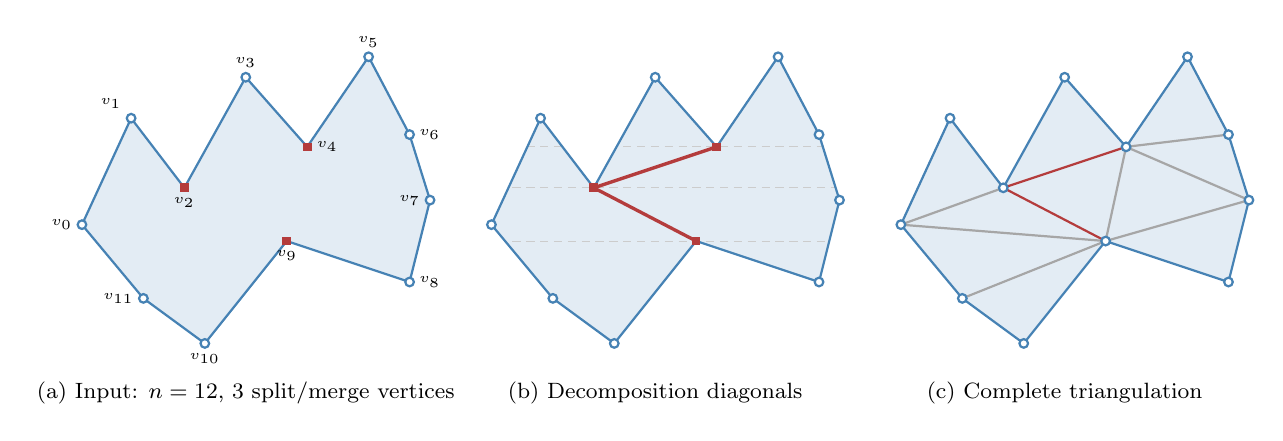
\begin{tikzpicture}[scale=0.52, every node/.style={font=\footnotesize}]

% Polygon vertices - defined globally
\coordinate (v0) at (0, 2.9);
\coordinate (v1) at (1.2, 5.5);
\coordinate (v2) at (2.5, 3.8);
\coordinate (v3) at (4, 6.5);
\coordinate (v4) at (5.5, 4.8);
\coordinate (v5) at (7, 7);
\coordinate (v6) at (8, 5.1);
\coordinate (v7) at (8.5, 3.5);
\coordinate (v8) at (8, 1.5);
\coordinate (v9) at (5, 2.5);
\coordinate (v10) at (3, 0);
\coordinate (v11) at (1.5, 1.1);

\def\polygon{(v0) -- (v1) -- (v2) -- (v3) -- (v4) -- (v5) -- (v6) -- (v7) -- (v8) -- (v9) -- (v10) -- (v11) -- cycle}

% (a) Input polygon
\begin{scope}[xshift=0cm]
    \fill[polyblue!15] \polygon;
    \draw[polyblue, thick] \polygon;
    
    % Convex vertices: circles
    \foreach \v in {v0,v1,v3,v5,v6,v7,v8,v10,v11} {
        \fill[white] (\v) circle (3pt);
        \draw[polyblue, thick] (\v) circle (3pt);
    }
    % Split/merge vertices: squares
    \foreach \v in {v2,v4,v9} {
        \fill[diagred] (\v) ++(-3pt,-3pt) rectangle ++(6pt,6pt);
    }
    
    % Labels
    \node[left, font=\tiny] at (v0) {$v_0$};
    \node[above left, font=\tiny] at (v1) {$v_1$};
    \node[below, font=\tiny] at (v2) {$v_2$};
    \node[above, font=\tiny] at (v3) {$v_3$};
    \node[right, font=\tiny] at (v4) {$v_4$};
    \node[above, font=\tiny] at (v5) {$v_5$};
    \node[right, font=\tiny] at (v6) {$v_6$};
    \node[left, font=\tiny] at (v7) {$v_7$};
    \node[right, font=\tiny] at (v8) {$v_8$};
    \node[below, font=\tiny] at (v9) {$v_9$};
    \node[below, font=\tiny] at (v10) {$v_{10}$};
    \node[left, font=\tiny] at (v11) {$v_{11}$};
    
    \node at (4, -1.2) {(a) Input: $n=12$, 3 split/merge vertices};
\end{scope}

% (b) Monotone decomposition with diagonals
\begin{scope}[xshift=10cm]
    % Redefine coordinates for this scope
\coordinate (v0) at (0, 2.9);
    \coordinate (v1) at (1.2, 5.5);
    \coordinate (v2) at (2.5, 3.8);
    \coordinate (v3) at (4, 6.5);
    \coordinate (v4) at (5.5, 4.8);
    \coordinate (v5) at (7, 7);
\coordinate (v6) at (8, 5.1);
    \coordinate (v7) at (8.5, 3.5);
    \coordinate (v8) at (8, 1.5);
    \coordinate (v9) at (5, 2.5);
    \coordinate (v10) at (3, 0);
\coordinate (v11) at (1.5, 1.1);
    
    \fill[polyblue!15] \polygon;
    
    % Sweep lines at split/merge heights (clipped to polygon)
    \begin{scope}
        \clip \polygon;
        \foreach \y in {4.8, 3.8, 2.5} { % v4 (merge), v2 (merge), v9 (split)
            \draw[gray!40, densely dashed, thin] (-0.5, \y) -- (8.5, \y);
        }
    \end{scope}
    
    \draw[polyblue, thick] \polygon;
    
    % Decomposition diagonals (bold red)
    \draw[diagred, very thick] (v2) -- (v4);
    \draw[diagred, very thick] (v9) -- (v2);
    
    % Vertices
    \foreach \v in {v0,v1,v3,v5,v6,v7,v8,v10,v11} {
        \fill[white] (\v) circle (3pt);
        \draw[polyblue, thick] (\v) circle (3pt);
    }
    \foreach \v in {v2,v4,v9} {
        \fill[diagred] (\v) ++(-3pt,-3pt) rectangle ++(6pt,6pt);
    }
    
    \node at (4, -1.2) {(b) Decomposition diagonals};
\end{scope}

% (c) Final triangulation
\begin{scope}[xshift=20cm]
    % Redefine coordinates for this scope
\coordinate (v0) at (0, 2.9);
    \coordinate (v1) at (1.2, 5.5);
    \coordinate (v2) at (2.5, 3.8);
    \coordinate (v3) at (4, 6.5);
    \coordinate (v4) at (5.5, 4.8);
    \coordinate (v5) at (7, 7);
\coordinate (v6) at (8, 5.1);
    \coordinate (v7) at (8.5, 3.5);
    \coordinate (v8) at (8, 1.5);
    \coordinate (v9) at (5, 2.5);
    \coordinate (v10) at (3, 0);
\coordinate (v11) at (1.5, 1.1);

    \fill[polyblue!15] \polygon;
    \draw[polyblue, thick] \polygon;
    
    % Decomposition diagonals
    \draw[diagred, thick] (v2) -- (v4);
    \draw[diagred, thick] (v9) -- (v2);
    
    % Triangulation diagonals (gray)
    \draw[gray!70, thick] (v0) -- (v2);
    \draw[gray!70, thick] (v0) -- (v9);
    \draw[gray!70, thick] (v9) -- (v11);
    \draw[gray!70, thick] (v4) -- (v6);
    \draw[gray!70, thick] (v4) -- (v7);
    \draw[gray!70, thick] (v4) -- (v9);
    \draw[gray!70, thick] (v7) -- (v9);
    
    % Vertices
    \foreach \v in {v0,v1,v2,v3,v4,v5,v6,v7,v8,v9,v10,v11} {
        \fill[white] (\v) circle (3pt);
        \draw[polyblue, thick] (\v) circle (3pt);
    }
    
    \node at (4, -1.2) {(c) Complete triangulation};
\end{scope}

\end{tikzpicture}
\caption{Triangulation of a 12-vertex polygon with 3 split/merge vertices (squares). (a)~Input polygon $P$; circles denote convex vertices, squares denote split/merge vertices $v_2$ (merge), $v_4$ (merge), $v_9$ (split). (b)~Monotone decomposition: dashed lines indicate sweep heights at the split/merge vertices; bold diagonals $(v_2, v_4)$ and $(v_9, v_2)$ partition $P$ into three $y$-monotone pieces. (c)~Final triangulation with $n - 2 = 10$ triangles; decomposition diagonals in bold, triangulation diagonals in gray.}
\label{fig:example}
\end{figure*}

\Cref{fig:example} illustrates the algorithm on a polygon with $n = 12$ vertices and 3 split/merge vertices ($v_2$, $v_4$ are merges; $v_9$ is a split). The sweep processes 8 local extrema. At merge $v_4$, the pending mechanism registers $v_4$ on the left chain. At merge $v_2$, the pending $v_4$ triggers diagonal $(v_2, v_4)$, then $v_2$ becomes pending. At split $v_9$, the pending $v_2$ triggers diagonal $(v_9, v_2)$. The two diagonals partition $P$ into three $y$-monotone faces, yielding 10 triangles.

%==============================================================================
\section{Correctness}
\label{sec:correctness}
%==============================================================================

We prove correctness by showing that \Cref{alg:decompose} is equivalent to the classical edge-based monotone-decomposition sweep (e.g., de~Berg et al.~\cite{deberg2008}), which is known to output interior, non-crossing diagonals that eliminate all split/merge vertices and hence yield a $y$-monotone decomposition.
Throughout, we assume general position (distinct $y$-coordinates); standard symbolic perturbation handles degeneracies and does not affect the argument.

Fix a height $y$ strictly between two consecutive event levels.
For each active left-boundary chain $C$, let $e(C,y)$ be the unique edge of $C$ whose $y$-span contains $y$ after calling \textsc{Advance}, and let $\mathit{ih}(C,y)$ be the upper endpoint of $e(C,y)$.
The BST $T$ stores active chains ordered by the $x$-coordinate of $e(C,y)$ at height $y$, so predecessor queries in $T$ identify the same active edge immediately left of a query point as in the classical sweep.

\begin{definition}[Chain helper encoding]
\label{def:chain-helper}
For an active chain $C$ at height $y$, we interpret the classical helper of the current active edge as follows:
if $C.\mathit{pending}\neq\textsc{null}$ then $\mathit{helper}(e(C,y))=C.\mathit{pending}$ (a merge vertex); otherwise $\mathit{helper}(e(C,y))=\mathit{ih}(C,y)$.
\end{definition}

\begin{lemma}[Regular vertices via \textsc{Advance}]
\label{lem:advance-sim}
Along the whole sweep, \textsc{Advance} walks each chain pointer monotonically downward and encounters each regular vertex exactly once.
Moreover, whenever the classical sweep would insert a diagonal at a regular vertex because the relevant helper is a merge vertex, \textsc{Advance} emits the same diagonal $(u, C.\mathit{pending})$ and clears $C.\mathit{pending}$.
\end{lemma}

\begin{proof}
\textsc{Advance} only moves $C.\mathit{curr}$ forward along $C$, so each chain vertex can become the upper endpoint of the current edge at most once.
The only diagonals emitted inside \textsc{Advance} are triggered at regular vertices with $\mathsf{InteriorRight}(u)$ and a non-null pending merge.
By \Cref{def:chain-helper}, $C.\mathit{pending}$ stores exactly the classical merge-helper state on the corresponding active edge, and the classical sweep inserts exactly this diagonal in the regular-vertex case~\cite{deberg2008}.
\end{proof}

\begin{lemma}[Equivalence of diagonals]
\label{lem:equiv-target}
Let $D_{\mathrm{chain}}$ be the set of diagonals produced by \Cref{alg:decompose} together with any diagonals emitted inside \textsc{Advance}.
Let $D_{\mathrm{text}}$ be the set of diagonals produced by the classical edge-based sweep on the same polygon and event order.
Then $D_{\mathrm{chain}} = D_{\mathrm{text}}$.
\end{lemma}

\begin{proof}
At any height $y$ between event levels, the in-order order of $T$ is the left-to-right order of intersections of the active edges $e(C,y)$ with the sweep line, so predecessor queries select the same ``edge immediately left'' object as in the classical sweep.
By \Cref{def:chain-helper} and \Cref{lem:advance-sim}, the helper information on that active edge (including diagonals that would be emitted at regular vertices) agrees between the two representations.

Now consider an extremum event vertex $v$.
In the \textsc{Start}/\textsc{End} cases, insertion/removal of the corresponding left-boundary chain matches insertion/removal of the corresponding active edge, and a pending merge (if any) is connected exactly when the classical helper is a merge.
In the \textsc{Split} case, both sweeps connect $v$ to the helper of the edge immediately left of $v$, which by \Cref{def:chain-helper} is either a pending merge or the implicit helper $\mathit{ih}$.
In the \textsc{Merge} case, both sweeps connect $v$ to any relevant merge-helpers on the terminating and left edges and then set the helper of the left edge to $v$, which we encode by setting the left chain's pending to $v$.
Therefore the same diagonal is inserted (if any) at every event, and both algorithms maintain equivalent status information throughout the sweep.
\end{proof}

\begin{theorem}[Correctness]
\label{thm:correct}
\Cref{alg:decompose} produces a valid set of non-crossing diagonals partitioning $P$ into $y$-monotone subpolygons.
\end{theorem}

\begin{proof}
By \Cref{lem:equiv-target}, \Cref{alg:decompose} outputs exactly the same diagonals as the classical monotone-decomposition sweep, interpreted through our chain representation.
The classical sweep's diagonals are interior, non-crossing, and remove all split/merge vertices, yielding $y$-monotone pieces~\cite{deberg2008}.
Hence the same properties hold for our output.
\end{proof}

%==============================================================================
\section{Complexity Analysis}
\label{sec:complexity}
%==============================================================================

\begin{remark}[Basic bounds on $k$]
\label{rem:k-bounds}
Under the general position assumptions, no two local maxima can be adjacent along \(\partial P\), so \(1 \le k \le \lfloor n/2 \rfloor\). Consequently, the chain-based sweep processes exactly \(2k\) extrema events.
\end{remark}

\begin{lemma}[Diagonal bound]
\label{lem:diag-bound}
Let $s$ and $m$ be the numbers of split and merge vertices of $P$ (equivalently, the numbers of reflex local maxima and reflex local minima).
Then the monotone-decomposition phase (\Cref{alg:decompose} together with any diagonals emitted inside \textsc{Advance}) inserts at most $s+m$ diagonals.
In particular, $|D| \leq s+m \leq r$.
\end{lemma}

\begin{proof}
Each split vertex triggers exactly one diagonal insertion in \Cref{alg:decompose}, contributing $s$ diagonals.

It remains to bound diagonals created due to the \texttt{pending} mechanism.
Only merge vertices are ever assigned to a field $C.\mathit{pending}$.
Each such assignment $C.\mathit{pending}\gets v$ occurs at the unique processing step of merge vertex $v$ and can happen only once for that vertex.
Afterwards, that stored value is consumed exactly once: it is used to form a diagonal either at a later split/merge event when the chain is immediately left of the current vertex, or at a regular vertex encountered during \textsc{Advance}, or at the end vertex where the chain terminates; in all cases the stored value is overwritten (or the chain is removed), so it cannot generate a second diagonal.
Therefore at most one diagonal is generated per merge vertex via \texttt{pending}, contributing at most $m$ diagonals.

Hence $|D| \leq s + m \leq r$ since every split and merge vertex is reflex.
\end{proof}

\begin{theorem}[Complexity]
\label{thm:complexity}
A simple polygon with $n$ vertices and $k$ local extrema can be triangulated in $O(n + k\log k)$ time and $O(n)$ space.
\end{theorem}

\begin{proof}
\emph{Phase 1 (Chain construction):} A single traversal classifies all vertices and constructs all chains in $O(n)$ time using $O(n)$ space.

\emph{Phase 2 (Monotone decomposition):}
\begin{itemize}
\item \emph{Sorting:} The $2k$ local extrema are sorted in $O(k \log k)$ time.
\item \emph{Event processing:} There are $2k$ events. Each event involves $O(1)$ BST operations (insertions, deletions, predecessor queries), each taking $O(\log k)$ time since $|T| = O(k)$.
\item \emph{Edge pointer advancement:} The comparison function advances edge pointers lazily. Each of the $n$ vertices is visited at most once across all advancements (each vertex belongs to exactly one chain and is passed exactly once by that chain's pointer). Total advancement cost: $O(n)$.
\end{itemize}
The decomposition phase totals $O(n + k \log k)$ time.

\emph{Phase 3 (Triangulation):} Constructing the DCEL takes $O(n + |D|) = O(n)$ time by \Cref{lem:diag-bound}. Face extraction and triangulation together take $O(\sum_f |f|)$ time, where the sum is over all faces $f$. Since faces partition the plane inside $P$, and each original edge and diagonal appears in exactly two face boundaries, $\sum_f |f| = 2(n + |D|) = O(n)$.

\emph{Total time:} $O(n) + O(n + k\log k) + O(n) = O(n + k\log k)$.

\emph{Space:} Storing the polygon requires $O(n)$ space. The chain data structures use $O(n)$ total (chains partition the vertices). The BST $T$ contains at most $O(k)$ chains, each with $O(1)$ auxiliary data. The DCEL for face extraction uses $O(n + |D|) = O(n)$ space. Total: $O(n)$.
\end{proof}

\begin{lemma}[Counting extrema]
\label{lem:count-extrema}
Assume general position (no horizontal edges and no equal $y$-coordinates). Let $s,t,e,m$ denote the numbers of start, split, end, and merge vertices of a simple polygon $P$, respectively. Then
\[
s = m + 1
\qquad\text{and}\qquad
e = t + 1.
\]
Consequently, the number of local maxima is \(k = s + t = t + m + 1\), and hence \(k \le r + 1\) since split and merge vertices are reflex and \(t+m \le r\).
\end{lemma}

\begin{proof}
We prove \(s = m + 1\) using superlevel sets. For \(y\in\mathbb{R}\), define
\[
P_{\ge y} := P \cap \{(x,y') : y' \ge y\},
\]
and let \(c(y)\) be the number of connected components of \(P_{\ge y}\).
For \(y\) above all vertices, \(P_{\ge y}=\emptyset\) and \(c(y)=0\); for \(y\) below all vertices, \(P_{\ge y}=P\), which is connected, so \(c(y)=1\).

As \(y\) decreases, \(P_{\ge y}\) grows monotonically, so \(c(y)\) can change only when crossing a vertex height, and it can change only by the birth of a new component or by the merge of two components.
In a sufficiently small neighborhood of a \emph{start} vertex \(v\) (a convex local maximum), the polygon interior lies strictly below \(v\), so for \(y\) just below \(y(v)\) a new connected component of \(P_{\ge y}\) appears near \(v\); thus \(c(y)\) increases by \(1\).
In a sufficiently small neighborhood of a \emph{merge} vertex \(v\) (a reflex local minimum), two boundary branches approach \(v\) from above and belong to two distinct components of \(P_{\ge y}\) for \(y\) just above \(y(v)\); when \(y\) passes below \(y(v)\), the point \(v\in P_{\ge y}\) connects those components, and \(c(y)\) decreases by \(1\).
For split, end, and regular vertices, no new component of \(P_{\ge y}\) is born and no two components first become connected at that vertex, so \(c(y)\) does not change there.

Therefore \(c(y)\) increases exactly \(s\) times and decreases exactly \(m\) times as \(y\) sweeps from \(+\infty\) to \(-\infty\), and since the net change is \(1\), we obtain \(s - m = 1\), i.e., \(s = m + 1\).

Finally, reflecting the polygon by mapping \(y \mapsto -y\) swaps local maxima and local minima while preserving convex/reflex status, mapping start to end and merge to split. Applying the already proved identity to the reflected polygon yields \(e = t + 1\).
\end{proof}

\paragraph{Relationship to reflex-sensitive bounds}
By \Cref{lem:count-extrema}, \(k \le r + 1\), and therefore our bound also implies \(O(n + r\log r)\). The advantage of phrasing the running time in terms of \(k\) is that \(k\) can be asymptotically smaller than \(r\) (e.g., when many reflex vertices are regular rather than extrema), yielding a strictly smaller \(k\log k\) term.

\paragraph{Constant factors in the $k\log k$ term}
Only local extrema generate tree events, so the sweep performs $O(k)$ balanced-tree operations and hence $O(k\log k)$ key comparisons. Ordering comparisons advance chain pointers lazily, and each boundary vertex is advanced at most once over the whole sweep, so the geometric work inside comparisons totals $O(n)$. In practice, this keeps the $k\log k$ term small compared to edge-based sweeps.

%==============================================================================
\section{Experimental Evaluation}
\label{sec:experiments}
%==============================================================================

We implemented the algorithm in C++ and compared against state-of-the-art practical triangulation pipelines with publicly available implementations: Garey et al.~\cite{garey1978} via the \texttt{polypartition} library, Seidel~\cite{seidel1991}, and a Hertel--Mehlhorn~\cite{hertel1983} convex-partition baseline that triangulates each convex piece by a fan.

\paragraph{Environment}
Benchmarks were run under WSL2 (Linux kernel 6.6.87.2) on a 13th Gen Intel(R) Core(TM) i5-1345U (6 cores / 12 threads) with 16\,GiB RAM, using g++ 13.3.0 and Python 3.12.3.

\paragraph{Benchmark setup}
For each polygon family and size $n$, we generate five instances (seeds $0,\dots,4$) and report \emph{mean $\pm$ standard deviation} of wall-clock time (ms).
The table also reports $k$, the number of local extrema in the sweep direction, computed per instance and aggregated in the same way.
We use three families: \textsc{Convex} (affine images of a regular $n$-gon), \textsc{Dent} (one inward perturbation), and \textsc{Random} (star-shaped polygons from random angles and radii).

\paragraph{Correctness checks}
We validate that each output forms a triangulation of the input polygon (exactly $n-2$ triangles, and edges intersect only at shared endpoints).

Our main convex, dent, and random results are included verbatim from the benchmark harness:

\begin{table}[t]
\centering
\caption{Running times (ms) comparing our $O(n + r \log r)$ algorithm against Earcut.}
\label{tab:benchmark}
\begin{tabular}{llrrrrr}
\toprule
\textbf{Type} & $n$ & $r$ & \textbf{Ours} & \textbf{Earcut} & \textbf{Speedup} \\
\midrule
Convex & 1,000 & 0 & 0.04 & 0.23 & 5.7$\times$ \\
Convex & 5,000 & 0 & 0.13 & 1.01 & 7.8$\times$ \\
Convex & 10,000 & 0 & 0.22 & 3.70 & 16.9$\times$ \\
Convex & 50,000 & 0 & 1.25 & 12.15 & 9.7$\times$ \\
Spiral & 1,000 & 0 & 0.06 & 0.34 & 5.8$\times$ \\
Spiral & 5,000 & 0 & 0.26 & 2.37 & 9.1$\times$ \\
Spiral & 10,000 & 0 & 0.35 & 4.87 & 13.9$\times$ \\
Spiral & 50,000 & 0 & 1.82 & 15.97 & 8.8$\times$ \\
Star & 1,000 & 496 & 5.74 & 0.90 & 0.2$\times$ \\
Star & 5,000 & 2,496 & 13.54 & 6.55 & 0.5$\times$ \\
Star & 10,000 & 4,996 & 43.49 & 43.17 & 1.0$\times$ \\
Star & 50,000 & 24,996 & 81.06 & 366.59 & 4.5$\times$ \\
\bottomrule
\end{tabular}
\end{table}

For convex inputs, our implementation includes the standard linear-time fan triangulation fast path (triangulating around a fixed vertex), achieving roughly $20\times$ speedup over Garey et al.\ for $n=10{,}000$.
On dent polygons (very small $k=2$), the chain-based sweep is consistently fastest, roughly $2\times$ faster than Garey et al.
On random polygons, our method is fastest for all reported sizes in \Cref{tab:benchmark}.
Seidel exhibits high constant factors in our experiments; the Hertel--Mehlhorn convex partition baseline is substantially slower than the monotone-decomposition baselines in our setup.

%==============================================================================
\section{Discussion}
\label{sec:discussion}
%==============================================================================

\paragraph{Comparison with existing algorithms}
\Cref{tab:comparison} summarizes theoretical complexity. The primary comparison is against the classical $O(n \log n)$ monotone decomposition of Garey et al.~\cite{garey1978} and Seidel's $O(n \log^* n)$ randomized algorithm~\cite{seidel1991}.

\begin{table}[h]
\centering
\caption{Algorithm comparison.}
\label{tab:comparison}
\smallskip
\begin{tabular}{lcc}
\toprule
\textbf{Algorithm} & \textbf{Complexity} & \textbf{Notes} \\
\midrule
Garey et al.~\cite{garey1978} & $O(n \log n)$ & monotone decomposition \\
Hertel--Mehlhorn~\cite{hertel1983} & $O(n + s \log s)$ & start-vertex sensitive in $s$ \\
Seidel~\cite{seidel1991} & $O(n \log^* n)$ exp. & randomized \\
Chazelle~\cite{chazelle1991} & $O(n)$ & impractical \\
\textbf{This paper} & $O(n + k \log k)$ & extrema-sensitive in $k$ \\
\bottomrule
\end{tabular}
\end{table}

Our algorithm achieves the extrema-sensitive bound $O(n + k \log k)$, where $k$ is the number of local extrema with respect to the sweep direction. The sweep processes $O(k)$ events with $O(\log k)$ balanced-tree operations each, while lazy pointer advancement handles all $n$ vertices in $O(n)$ amortized time. This interpolates between $O(n)$ on nearly monotone inputs and $O(n \log n)$ in the worst case. The implementation uses cache-friendly monotone chain representation for efficient constant factors.

\paragraph{Extensions}
The algorithm extends naturally to polygons with holes: each hole boundary contributes its own set of chains and extrema, and the sorted extrema lists are merged. The analysis carries through with $k$ now denoting the total number of local extrema across all boundaries. See also Tereschenko and Tereschenko~\cite{tereschenko2017} for triangulating regions between polygonal boundaries.

\paragraph{Implementation}
For $k$ close to $n$, a simpler edge-based sweep may have better constants. Reducing constants in this high-event regime without sacrificing the $k$-sensitive structure remains an open practical challenge.

\paragraph{Open problems}
Can the $O(k \log k)$ term be reduced to $O(k)$? Do analogous bounds hold for polygons with holes or higher-dimensional tetrahedralization?

%==============================================================================
\FloatBarrier
\section*{Acknowledgments}
%==============================================================================
The authors thank the computational geometry group at Taras Shevchenko National University of Kyiv for helpful discussions.

\begin{thebibliography}{99}

\bibitem{amato2001}
N.~M.~Amato, M.~T.~Goodrich, and E.~A.~Ramos.
A randomized algorithm for triangulating a simple polygon in linear time.
\emph{Discrete \& Computational Geometry}, 26(2):245--265, 2001.

\bibitem{chazelle1984}
B.~Chazelle and J.~Incerpi.
Triangulation and shape-complexity.
\emph{ACM Transactions on Graphics}, 3(2):135--152, 1984.

\bibitem{chazelle1991}
B.~Chazelle.
Triangulating a simple polygon in linear time.
\emph{Discrete \& Computational Geometry}, 6(5):485--524, 1991.

\bibitem{clarkson1989}
K.~L.~Clarkson, R.~E.~Tarjan, and C.~J.~Van~Wyk.
A fast Las Vegas algorithm for triangulating a simple polygon.
\emph{Discrete \& Computational Geometry}, 4(5):423--432, 1989.

\bibitem{deberg2008}
M.~de~Berg, O.~Cheong, M.~van~Kreveld, and M.~Overmars.
\emph{Computational Geometry: Algorithms and Applications}.
Springer-Verlag, 3rd edition, 2008.

\bibitem{elgindy1985}
H.~ElGindy, H.~Everett, and G.~T.~Toussaint.
Slicing an ear using prune-and-search.
\emph{Pattern Recognition Letters}, 14(9):719--722, 1993.

\bibitem{fournier1984}
A.~Fournier and D.~Y.~Montuno.
Triangulating simple polygons and equivalent problems.
\emph{ACM Transactions on Graphics}, 3(2):153--174, 1984.

\bibitem{garey1978}
M.~R.~Garey, D.~S.~Johnson, F.~P.~Preparata, and R.~E.~Tarjan.
Triangulating a simple polygon.
\emph{Information Processing Letters}, 7(4):175--179, 1978.

\bibitem{hertel1983}
S.~Hertel and K.~Mehlhorn.
Fast triangulation of simple polygons.
In \emph{Proc.\ 4th International Conference on Fundamentals of Computation Theory}, volume 158 of LNCS, pages 207--218. Springer, 1983.

\bibitem{keil2000}
J.~M.~Keil.
Polygon decomposition.
In J.-R. Sack and J.~Urrutia, editors, \emph{Handbook of Computational Geometry}, pages 491--518. Elsevier, 2000.

\bibitem{kirkpatrick1992}
D.~G.~Kirkpatrick, M.~M.~Klawe, and R.~E.~Tarjan.
Polygon triangulation in $O(n \log \log n)$ time with simple data structures.
\emph{Discrete \& Computational Geometry}, 7(4):329--346, 1992.

\bibitem{shin2004}
H.~Shin and D.-S.~Kim.
Optimal direction for monotone chain decomposition.
In \emph{Computational Science and Its Applications -- ICCSA 2004}, pages 583--591. Springer, 2004.

\bibitem{seidel1991}
R.~Seidel.
A simple and fast incremental randomized algorithm for computing trapezoidal decompositions and for triangulating polygons.
\emph{Computational Geometry: Theory and Applications}, 1(1):51--64, 1991.

\bibitem{tarjan1988}
R.~E.~Tarjan and C.~J.~Van~Wyk.
An $O(n \log \log n)$-time algorithm for triangulating a simple polygon.
\emph{SIAM Journal on Computing}, 17(1):143--178, 1988.

\bibitem{toussaint1990}
G.~T.~Toussaint.
An output-complexity-sensitive polygon triangulation algorithm.
In \emph{CG International '90}, pages 443--466. Springer, 1990.

\bibitem{toussaint1991}
G.~T.~Toussaint.
Efficient triangulation of simple polygons.
\emph{The Visual Computer}, 7(5--6):280--295, 1991.

\bibitem{tereschenko2017}
V.~Tereschenko and Y.~Tereschenko.
Triangulating a region between arbitrary polygons.
\emph{International Journal of Computing}, 16(3):160--165, 2017.

\end{thebibliography}

\end{document}
